\documentclass[11pt]{article}
\usepackage[margin=1in]{geometry}
\usepackage{graphicx}
\usepackage{hyperref}
\usepackage{parskip}
\usepackage{appendix}

\title{UAVSAR $\Delta$SWE Retrievals at Mores Creek Summit:\\
\large Selected InSAR pairs for sub-km precipitation-pattern input to snow models}
\author{HP Marshall, Boise State University}
\date{September 2026}

\begin{document}
\maketitle

\section{Purpose and data context}

Snow models are usually forced with precipitation fields far coarser than the sub-km
accumulation patterns that terrain imposes. L-band repeat-pass InSAR measures the phase
change caused by SWE gained between two flights, at meter-scale resolution. This report
summarizes a pilot at Mores Creek Summit (MCS), Idaho, that turns 22 SnowEx UAVSAR
interferometric pairs (winters 2019--20 and 2020--21, lines 05208 and 23205) into
$\Delta$SWE maps, evaluates them against airborne lidar snow depth and the in-domain
SNOTEL, and selects the pairs most useful for defining the sub-km precipitation pattern.
Figure~\ref{fig:snotel} places every UAVSAR flight and both QSI lidar surveys on the
SNOTEL SWE record.

\begin{figure}[h]
\centering
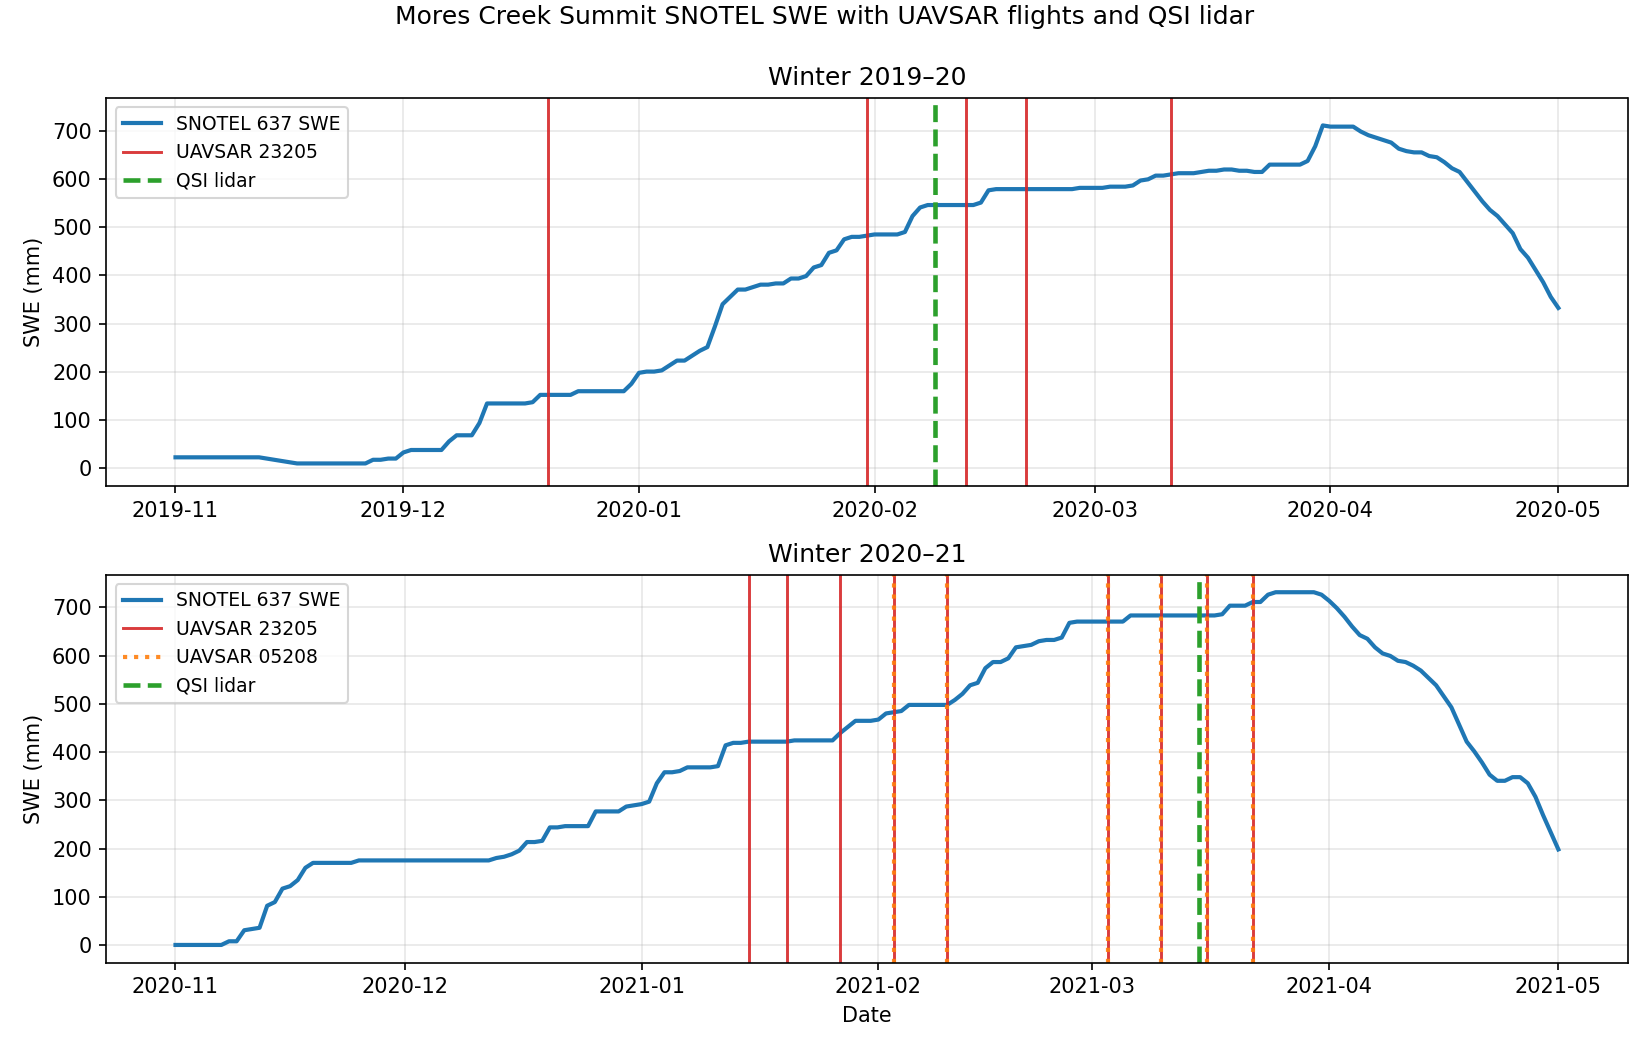
\includegraphics[width=\textwidth]{snotel_swe_flights.png}
\caption{Mores Creek Summit SNOTEL (637:ID:SNTL) daily SWE for the two campaign winters.
Vertical lines: UAVSAR flights (line 23205 solid red, line 05208 dotted orange; the two
lines flew the same days in 2021). Dashed green: QSI lidar snow-depth surveys
(2020-02-09 and 2021-03-15).}
\label{fig:snotel}
\end{figure}

\section{Recommended pairs}

Table~\ref{tab:top} lists the five ranked pairs plus one additional example. The rank
criterion is the mean (over four polarizations) Pearson correlation at 90\,m between the
pair's $\Delta$SWE map and the season-matched lidar snow depth, restricted to pairs whose
interval contains real snowfall (SNOTEL $\Delta$SWE $\ge$ +10\,mm) with adequate valid
area ($n_{90} \ge 500$ cells). Pair 4 fails only the snowfall gate: a near-zero-change
interval whose retrieval still tracks the snowpack pattern ($r = +0.49$ against the lidar
it brackets), making it a clean null/redistribution test case for a model.

\begin{table}[h]
\centering
\caption{Top 5 pairs for precipitation-pattern input, plus the zero-change example.
$r$ vs lidar is the polarization-mean correlation with the season-matched QSI snow
depth at 90\,m; cross-pol is the mean inter-polarization correlation of the retrieval.}
\label{tab:top}
\medskip
\resizebox{\textwidth}{!}{\begin{tabular}{cclllrrrr}
\hline
label & rank & pair & line & dates & SNOTEL $\Delta$SWE (mm) & $r$ vs lidar & cross-pol & $n_{90}$ \\
\hline
\textbf{A} & 1 & 8 & 05208 & 2021-02-10 $\rightarrow$ 2021-03-03 & +173 & +0.637 & +0.89 & 3220 \\
\textbf{B} & 2 & 2 & 23205 & 2021-03-10 $\rightarrow$ 2021-03-22 & +28 & +0.577 & +0.95 & 3685 \\
\textbf{C} & 3 & 1 & 23205 & 2021-03-16 $\rightarrow$ 2021-03-22 & +28 & +0.483 & +0.88 & 3594 \\
\textbf{D} & 4 & 5 & 23205 & 2021-03-03 $\rightarrow$ 2021-03-16 & +13 & +0.466 & +0.90 & 3729 \\
\textbf{E} & 5 & 6 & 05208 & 2021-03-03 $\rightarrow$ 2021-03-10 & +13 & +0.454 & +0.94 & 4413 \\
\hline
\textbf{F} & -- & 4 & 23205 & 2021-03-10 $\rightarrow$ 2021-03-16 & +0 & +0.486 & +0.95 & 3819 \\
\hline
\end{tabular}
}
\end{table}

Two features strengthen the top choices: pair 8 correlates nearly equally with the 2020
lidar ($+0.650$) and the 2021 lidar ($+0.637$), evidence that the accumulation pattern it
captures is the persistent, terrain-controlled one a model precipitation field should
inherit; and pairs 5/6 sample the same early-March snowfall from opposite headings,
giving a built-in cross-view consistency check.

\section{Processing steps}

\subsection{Site cropping and the canonical grid}
All products are cropped to the MCS lidar footprint and expressed on one canonical grid:
3\,m, UTM 11N (EPSG:32611), 2801 $\times$ 2624 cells, derived from the native 0.5\,m QSI
lidar grid. Everything downstream --- lidar, phase, coherence, incidence angle,
atmosphere, retrievals --- shares this grid, so no resampling is needed at analysis time.

\subsection{Regridding to 3 m}
Lidar products (snow depth, DTM, DSM, CHM) are block-averaged 0.5\,m~$\to$~3\,m. UAVSAR
ground-projected products are reprojected from their native equiangular grid: coherence
and unwrapped phase bilinearly, and \emph{wrapped} phase in the complex domain (averaging
real and imaginary parts separately) so that phase wrapping is respected.

\subsection{Atmospheric correction}
For each of the 20 flights, ERA5 pressure-level reanalysis at the acquisition hour gives
a refractivity profile from which the two-way phase delay is integrated \emph{below the
aircraft altitude} ($\sim$12.5\,km --- UAVSAR flies inside the atmosphere, so the
standard satellite formulation is referenced to the aircraft, not the model top), mapped
through the local incidence angle. Per-pair differences (\texttt{atm\_delay\_diff}) are
subtracted from the unwrapped phase.

\subsection{Local incidence angle}
Per-line local incidence angle comes from the JPL Stack look vectors (.lkv/.llh files)
combined with the 2023-02-09 lidar DTM, mosaicked across the three along-track segments
and geocoded directly onto the canonical grid. Grazing and back-facing terrain
($\cos(\mathrm{LIA}) \le 0.05$) is masked.

\subsection{Unwrapping of pairs without an ASF product}
Five pairs (9, 12, 14, 20, 21) ship no unwrapped phase from ASF. Their wrapped
interferograms were multilooked 5$\times$5 (to 15\,m), unwrapped with SNAPHU
(smooth-cost, MCF initialization, coherence-weighted), and restored to 3\,m by choosing,
at every pixel, the $2\pi$ branch of the original wrapped phase nearest the upsampled
unwrapped field --- exact rewrap consistency by construction. Caveat: disconnected
unwrapped components carry independent phase constants (most relevant for the
low-coherence 2020 pairs 20 and 21).

\subsection{Phase ramp removal}
Pair 8 (05208, 2021-02-10~$\to$~03-03, the 173\,mm storm sequence) carried a residual
long-wavelength tilt ($\sim$0.15\,rad\,km$^{-1}$), typical of small aircraft-motion /
baseline errors. The correction fits $\varphi = a + bx + cy + d\,z(\mathrm{DEM})$ at
90\,m and removes only the planar part; the elevation-correlated term
($+0.34$\,rad per 100\,m) is deliberately \emph{kept}, since orographic accumulation is
itself elevation-correlated. The pair's lidar correlation improved from $+0.635$ to
$+0.672$.

\subsection{$\Delta$SWE inversion and validation}
Corrected phase is inverted with the Guneriussen et al.\ (2001) dry-snow relation using
the real per-pixel incidence angle and new-snow density 250\,kg\,m$^{-3}$, masked at
coherence $< 0.35$, and anchored so the 90\,m window at the MCS SNOTEL matches the
station's interval $\Delta$SWE (SNOTEL is therefore a \emph{reference}, not an
independent check). Four validations: (i) phase-closure triangles, RMS 0.5--1.6\,rad
$\approx$ 7--21\,mm w.e.\ for ASF-product triangles (24--31\,mm where a custom-unwrapped
pair participates) --- small against 50--170\,mm storm signals; (ii) cross-polarization
consistency $r = 0.71$--$0.96$ for the well-observed pairs; (iii) SNOTEL anchor
diagnostics (offsets and interval densities logged per pair); (iv) lidar comparisons ---
the 2021-03-15 survey falls inside pair 4's interval ($r = +0.51$ HH), and the top-ranked
pairs reach $r = +0.45$ to $+0.65$.

\section{Deliverables}

\begin{itemize}
\item \texttt{mcs\_top\_pairs\_subset.nc} (1.2\,GB NetCDF4): the six pairs of
      Table~\ref{tab:top} in rank order (\texttt{rank\_note} coordinate), with
      $\Delta$SWE, coherence, unwrapped phase and atmospheric correction per pair, plus
      the two QSI snow-depth surveys, the DEM, and both lines' incidence angle. Format
      details in the companion user guide.
\item \texttt{mcs\_zarr\_userguide.pdf}: complete format specification of the master
      datacube and of the subset file.
\end{itemize}

\appendix
\section{Full pair ranking}

\begin{table}[h]
\centering
\caption{All 22 pairs: polarization-mean correlation of $\Delta$SWE with each lidar
survey at 90\,m, SNOTEL interval $\Delta$SWE (mm), valid 90\,m cells, cross-polarization
consistency, and gate/provenance notes. Ranking uses the season-matched lidar column.}
\label{tab:appendix}
\medskip
\resizebox{\textwidth}{!}{\begin{tabular}{cllrrrrrl}
\hline
pair & line & dates & SNOTEL & $r$ 2020 & $r$ 2021 & $n_{90}$ & cross-pol & notes \\
\hline
0 & 05208 & 2021-03-16 $\rightarrow$ 2021-03-22 & +28 & +0.061 & +0.185 & 3157 & +0.82 & rank 11 \\
1 & 23205 & 2021-03-16 $\rightarrow$ 2021-03-22 & +28 & +0.229 & +0.483 & 3594 & +0.88 & rank 3 \\
2 & 23205 & 2021-03-10 $\rightarrow$ 2021-03-22 & +28 & +0.362 & +0.577 & 3685 & +0.95 & rank 2 \\
3 & 05208 & 2021-03-10 $\rightarrow$ 2021-03-16 & +0 & -0.210 & -0.292 & 4415 & +0.95 & no snowfall \\
4 & 23205 & 2021-03-10 $\rightarrow$ 2021-03-16 & +0 & +0.370 & +0.486 & 3819 & +0.95 & zero-change example, no snowfall \\
5 & 23205 & 2021-03-03 $\rightarrow$ 2021-03-16 & +13 & +0.238 & +0.466 & 3729 & +0.90 & rank 4 \\
6 & 05208 & 2021-03-03 $\rightarrow$ 2021-03-10 & +13 & +0.335 & +0.454 & 4413 & +0.94 & rank 5 \\
7 & 23205 & 2021-03-03 $\rightarrow$ 2021-03-10 & +13 & -0.028 & +0.170 & 3679 & +0.91 & rank 12 \\
8 & 05208 & 2021-02-10 $\rightarrow$ 2021-03-03 & +173 & +0.650 & +0.637 & 3220 & +0.89 & rank 1 \\
9 & 23205 & 2021-02-10 $\rightarrow$ 2021-03-03 & +173 & +0.257 & +0.318 & 3723 & +0.87 & rank 6, SNAPHU unwrap \\
10 & 05208 & 2021-02-03 $\rightarrow$ 2021-02-10 & +15 & +0.123 & -0.142 & 4394 & +0.96 & rank 18 \\
11 & 23205 & 2021-02-03 $\rightarrow$ 2021-02-10 & +15 & +0.187 & +0.109 & 3157 & +0.94 & rank 14 \\
12 & 23205 & 2021-01-27 $\rightarrow$ 2021-02-10 & +58 & +0.289 & +0.140 & 3408 & +0.41 & rank 13, SNAPHU unwrap \\
13 & 23205 & 2021-01-27 $\rightarrow$ 2021-02-03 & +43 & +0.251 & +0.255 & 653 & +0.89 & rank 8 \\
14 & 23205 & 2021-01-20 $\rightarrow$ 2021-02-03 & +61 & -0.027 & -0.046 & 3191 & +0.67 & rank 16, SNAPHU unwrap \\
15 & 23205 & 2021-01-20 $\rightarrow$ 2021-01-27 & +18 & -0.050 & +0.002 & 3727 & +0.72 & rank 15 \\
16 & 23205 & 2021-01-15 $\rightarrow$ 2021-01-27 & +18 & -0.402 & -0.467 & 3209 & +0.92 & rank 19 \\
17 & 23205 & 2021-01-15 $\rightarrow$ 2021-01-20 & +0 & -0.309 & -0.434 & 3695 & +0.82 & no snowfall \\
18 & 23205 & 2020-02-21 $\rightarrow$ 2020-03-11 & +30 & +0.313 & +0.550 & 2795 & +0.94 & rank 7 \\
19 & 23205 & 2020-02-13 $\rightarrow$ 2020-02-21 & +33 & +0.189 & +0.389 & 2658 & +0.71 & rank 10 \\
20 & 23205 & 2020-01-31 $\rightarrow$ 2020-02-13 & +64 & -0.080 & -0.145 & 1657 & +0.53 & rank 17, SNAPHU unwrap \\
21 & 23205 & 2019-12-20 $\rightarrow$ 2020-01-31 & +330 & +0.222 & +0.291 & 858 & +0.35 & rank 9, SNAPHU unwrap \\
\hline
\end{tabular}
}
\end{table}

\end{document}
